78. \begin{figure}[ht!]
\center{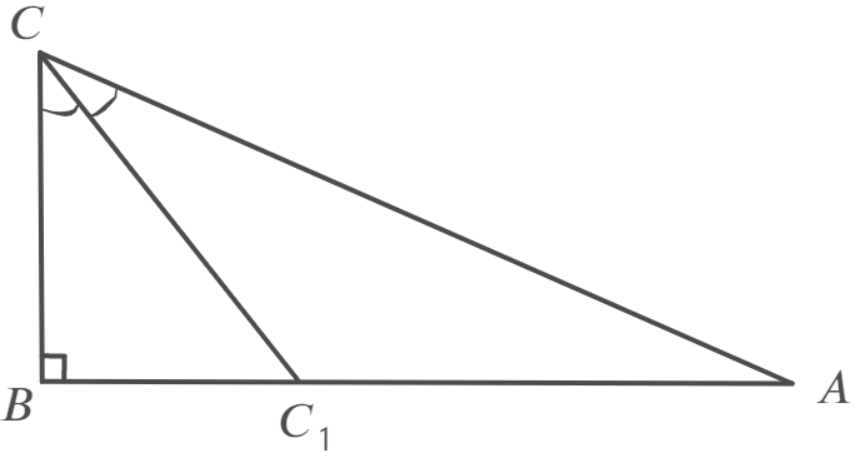
\includegraphics[scale=0.35]{g78.png}}
\end{figure}\\
В прямоугольном треугольнике $BCC_1$ катет $BC_1=8$см в 2 раза меньше гипотенузы $CC_1=16$см, значит $\angle BCC_1=30^\circ.$ Так как $CC_1$ биссектриса, $\angle C=2\cdot30^\circ=60^\circ,$ а значит $\angle A=90^\circ-60^\circ=30^\circ$ и внешний угол при вершине $A$ равен $180^\circ-30^\circ=150^\circ.$\\
